
\section{Overview about Transfer Learning Attack} % Sections are added in order to organize your presentation into discrete blocks, all sections and subsections are automatically output to the table of contents as an overview of the talk but NOT output in the presentation as separate slides

%------------------------------------------------

\begin{frame}{What is Transfer Learning?}
    \begin{itemize}
     \item Transfer Learning is a method reuse models trained on a large dataset in the source domain to solve problems in the target domain – where data is often scarce.
    \item This method saves time, costs and improves system efficiency.
    \end{itemize}
   \begin{figure}[h]
       \centering
       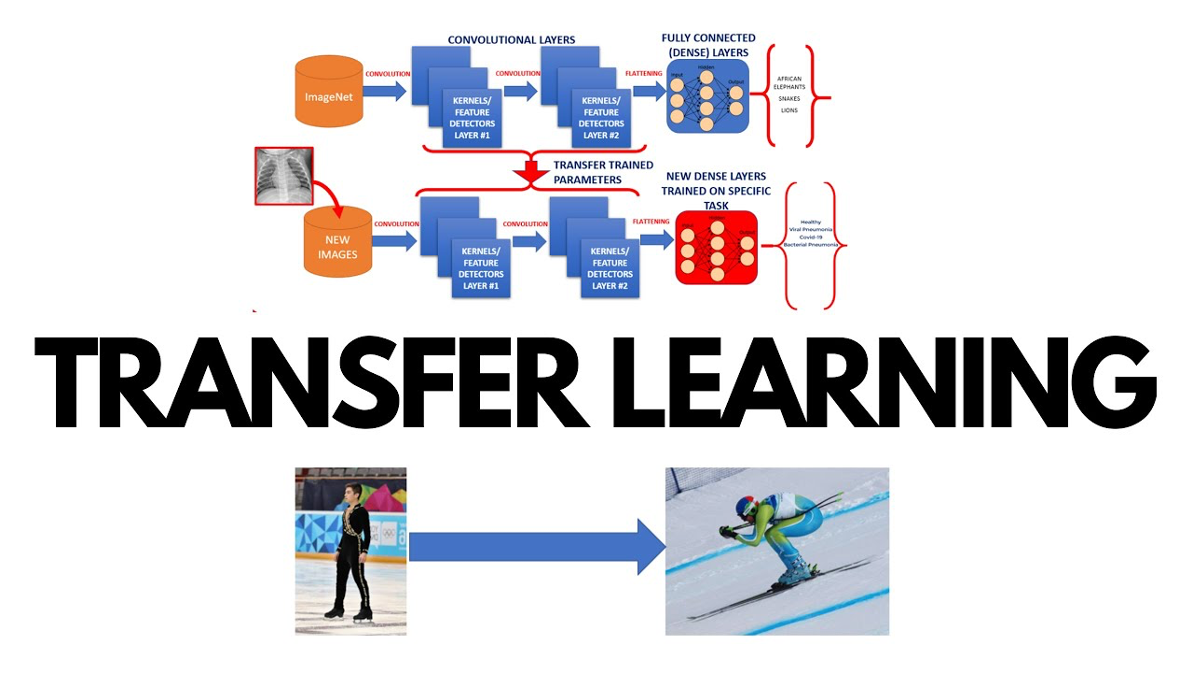
\includegraphics[width=0.5\textwidth]{img/what-is.png}
       \caption{Transfer Learning}
       \label{fig:what-is}
   \end{figure}
\end{frame}
% %------------------------------------------------
\begin{frame}{Why is Transfer Learning Attack dangerous?}
    \begin{figure}
        \centering
        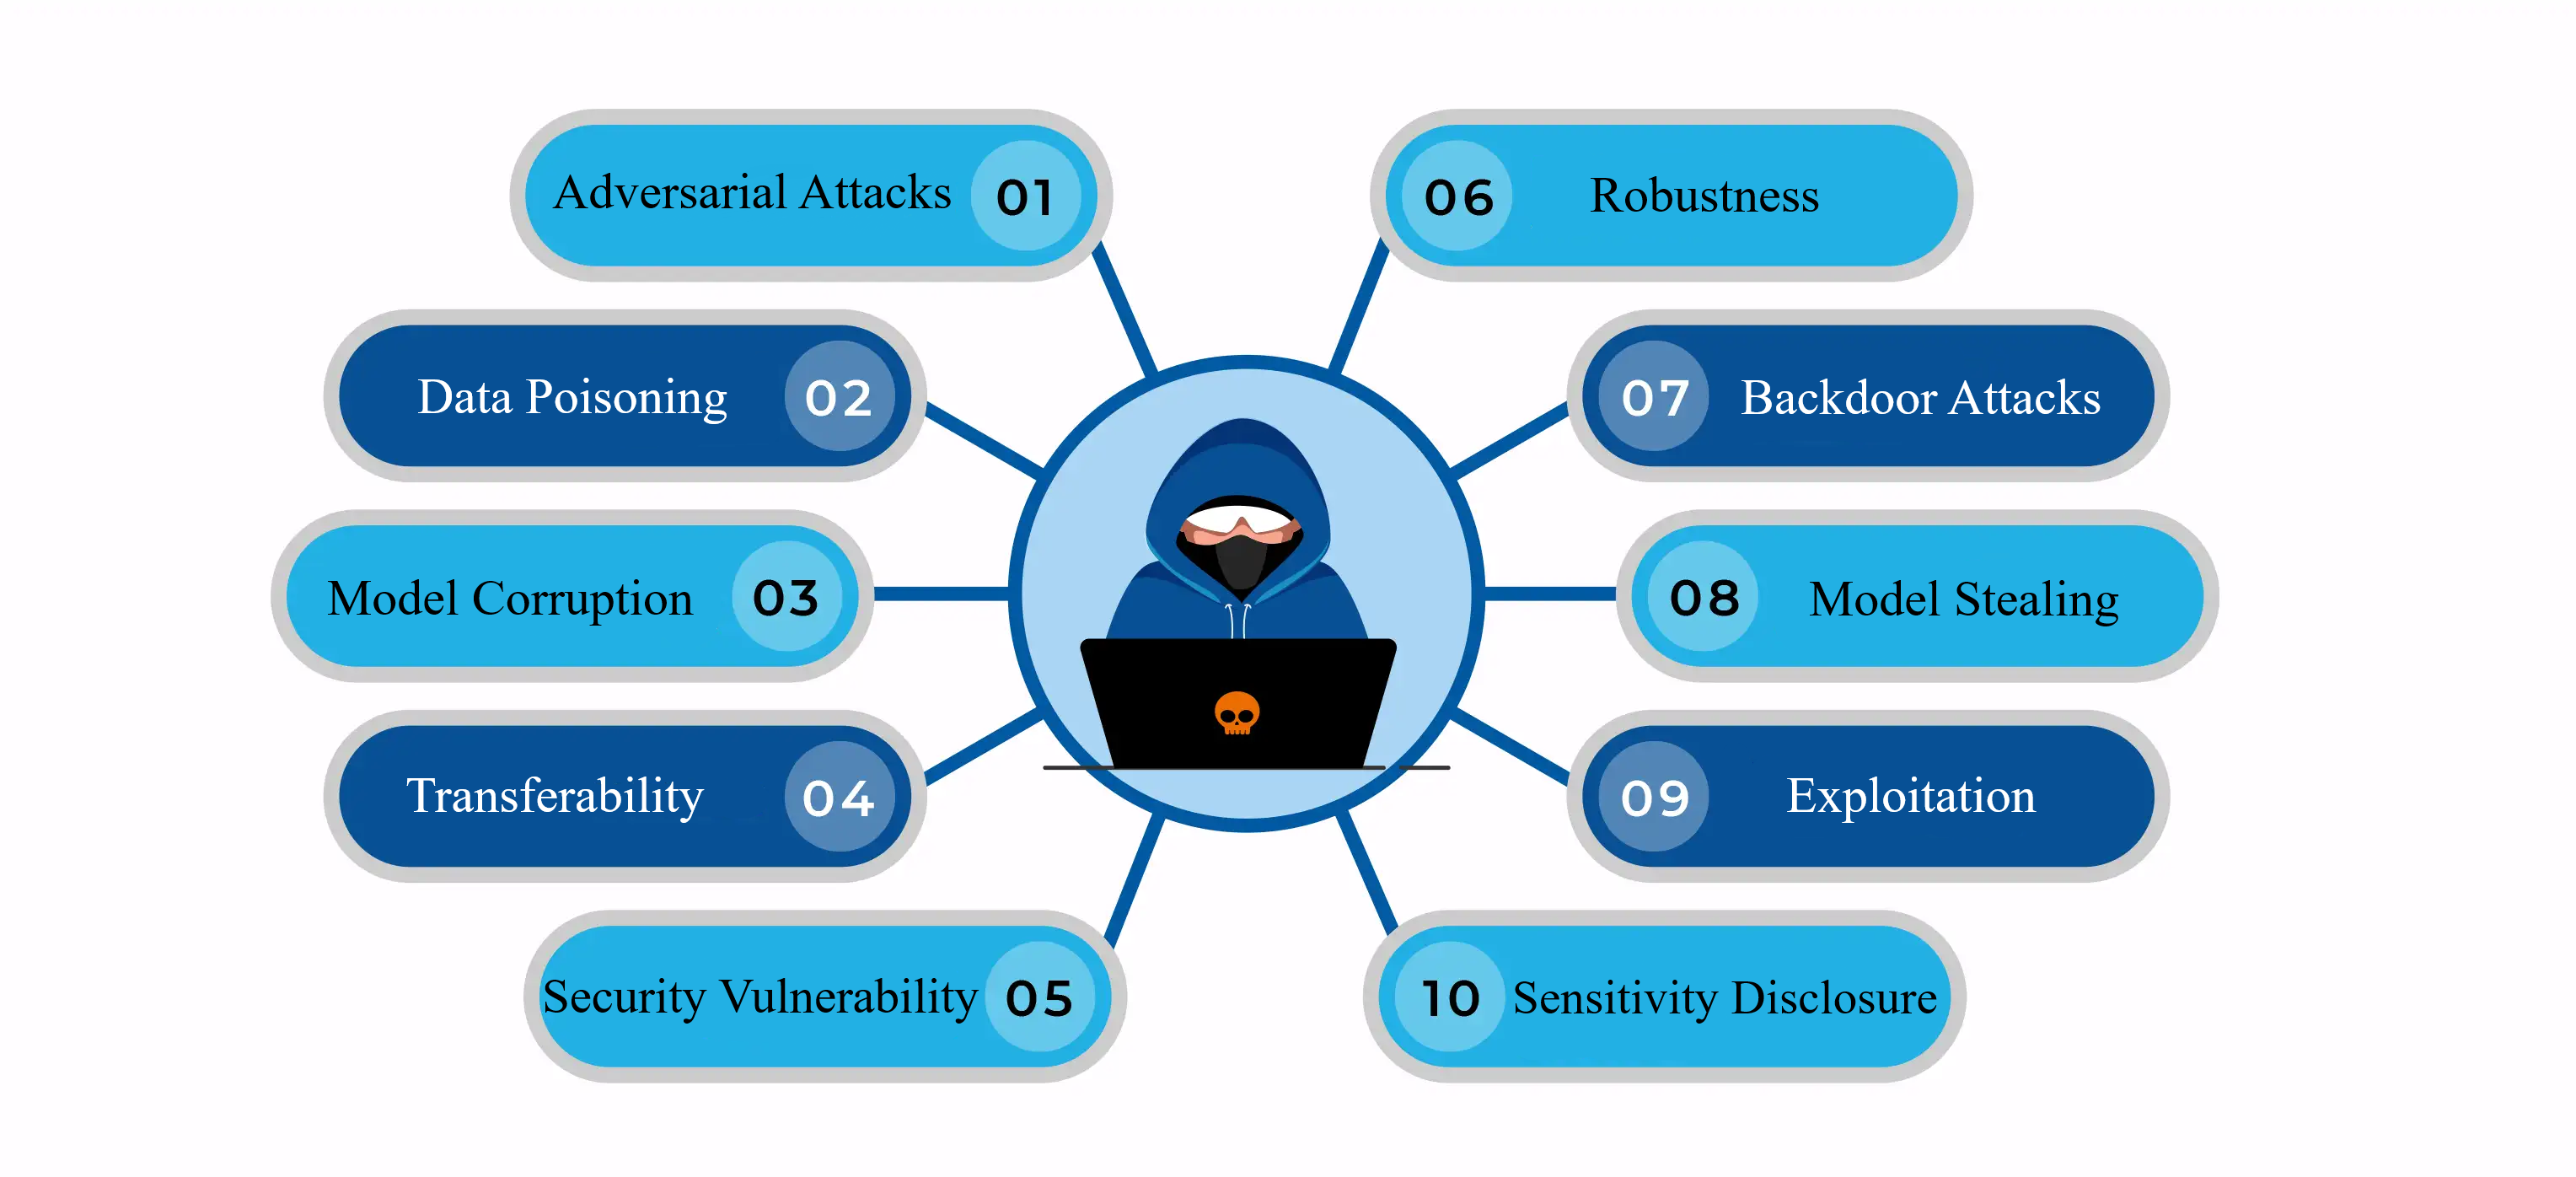
\includegraphics[width=0.8\linewidth]{img/Why.png}
        \caption{The dangers of Transfer Learning Attacks}
        \label{fig:why}
    \end{figure}

\end{frame}
% %------------------------------------------------
\begin{frame}{When Does Transfer Learning Attack Happen?}
    \begin{itemize}
        \item \textbf{Model Pre-Training:} 
        Attackers train a model with backdoored data and upload it to public repositories.
        \item \textbf{Re-Training:} 
        Users re-train the model on their clean dataset, unaware of the embedded backdoor.
        \item \textbf{Deployment:} 
        The compromised model is deployed, and triggers (e.g., manipulated traffic signs) exploit its vulnerabilities.
    \end{itemize}
    \begin{figure}[h]
        \centering
        
        \begin{minipage}{0.4\textwidth} % Adjust width to fit the image
            \centering
            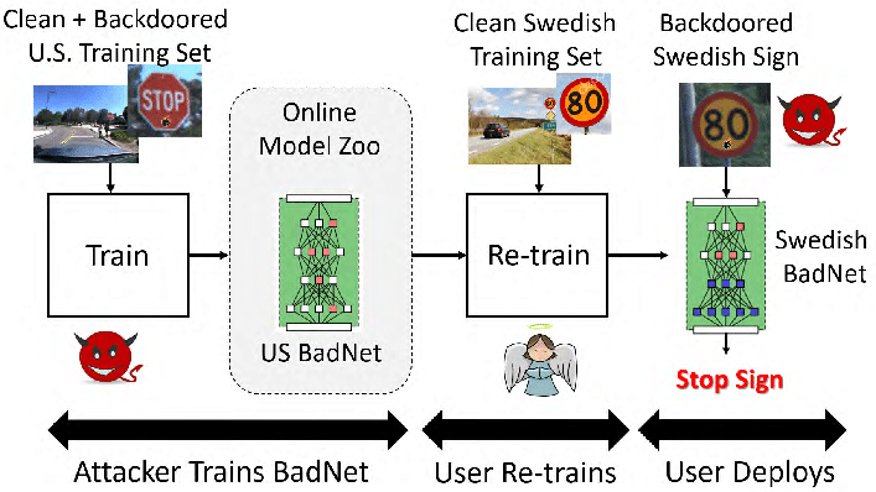
\includegraphics[width=\textwidth]{img/when-is.png} % Replace with actual image path
        \end{minipage}
        \begin{minipage}{0.35\textwidth} % Adjust width as needed
            \caption{Scenarios of Transfer Learning Attack.}
            \label{fig:transfer-attack}
        \end{minipage}%
    \end{figure}

\end{frame}

%------------------------------------------------
\begin{frame}{Where does Transfer Learning Attack occur?}
    \begin{itemize}
        \item Transfer Learning Attacks can target multiple critical domains where AI and machine learning models are widely used.
    \end{itemize}

    \begin{columns}[T] % Top alignment for consistency
        % Left Column
        \column{0.5\textwidth}
        \textbf{\large Transportation:}
        \begin{itemize}
            \item Adversarial attacks can mislead self-driving cars.
           %  \item Example: Modifying a traffic sign from "STOP" to "GO."
        \end{itemize}
        \begin{figure}[h]
            \centering
            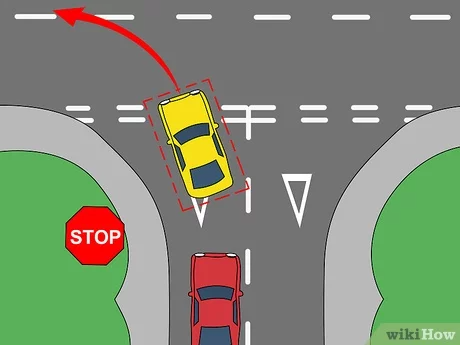
\includegraphics[width=0.5\linewidth]{img/StopToGo.png}
            % \caption{Adversarial Attack in Transportation}
            % \label{fig:StopToGo}
        \end{figure}

        % Right Column
        \column{0.5\textwidth}
        \begin{itemize}
            \item \textbf{\large Healthcare:}
            \begin{itemize}
                \item Manipulating medical image classifiers to misdiagnose conditions.
                % \item Example: Falsifying X-ray results to miss critical illnesses.
            \end{itemize}
        \end{itemize}
        \begin{figure}[h]
            \centering
            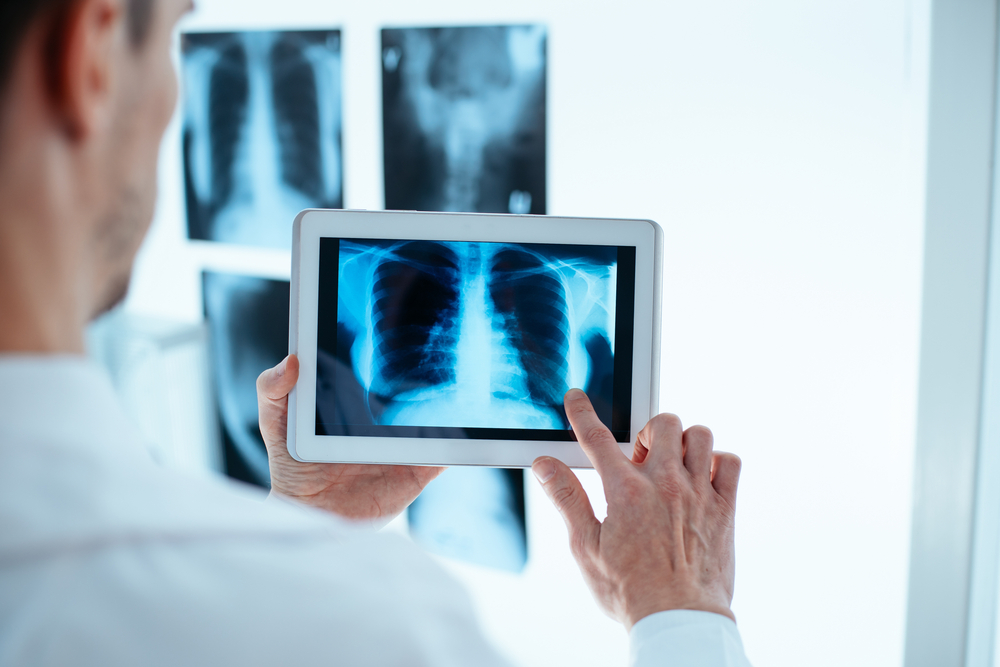
\includegraphics[width=0.55\linewidth]{img/X-ray_results.png}
            % \caption{Adversarial Attack in Transportation}
            % \label{fig:StopToGo}
        \end{figure}
    \end{columns}
\end{frame}

% %------------------------------------------------
\begin{frame}{Where does Transfer Learning Attack occur?}
    \begin{itemize}
        \item Transfer Learning Attacks can target multiple critical domains where AI and machine learning models are widely used.
    \end{itemize}

    \begin{columns}
        \column{0.5\textwidth}
        \begin{itemize}
            \item \textbf{\large Finance:}
            \begin{itemize}
                \item Exploiting fraud detection models by injecting poisoned data.
                % \item Example: Approving illegitimate transactions.
            \end{itemize}
            \begin{figure}[h]
                \centering
                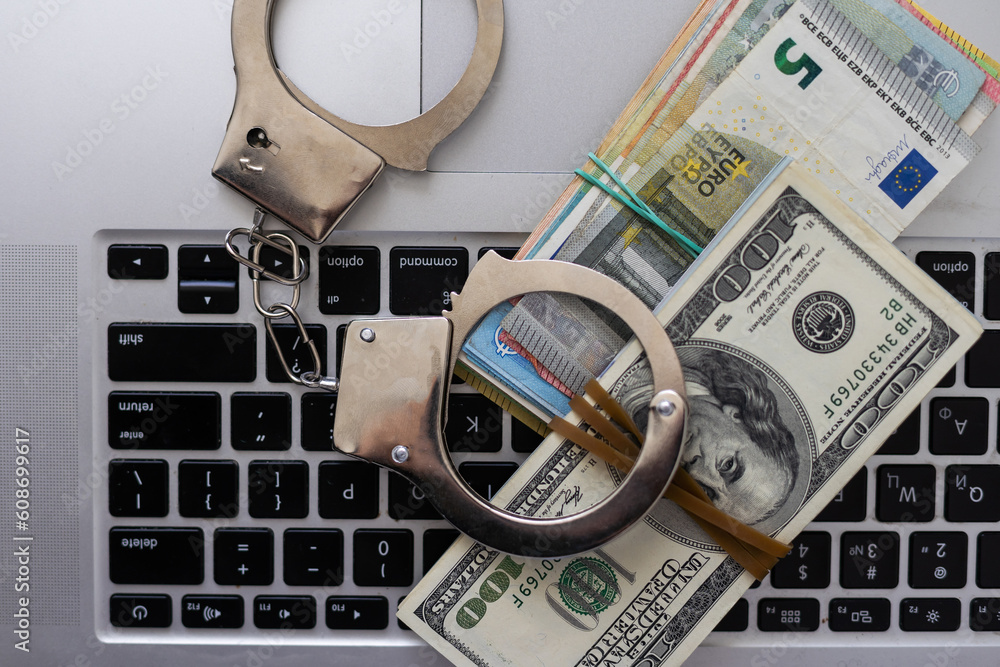
\includegraphics[width=0.7\linewidth]{img/Approving_illegitimate_transactions.png}
                % \caption{Enter Caption}
                % \label{fig:enter-label}
            \end{figure}
        \end{itemize}

        \column{0.5\textwidth}
        \begin{itemize}
            \item \textbf{\large Security:}
            \begin{itemize}
                \item Circumventing intrusion detection systems.
                % \item Example: Using adversarial inputs to bypass firewall defenses.
            \end{itemize}
            \begin{figure}
                \centering
                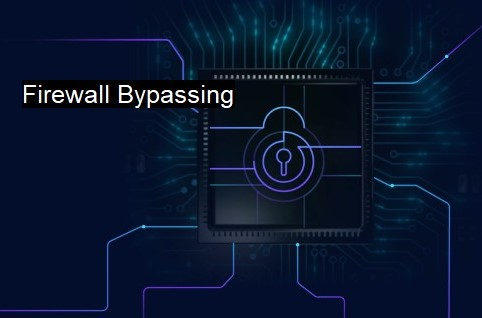
\includegraphics[width=0.7\linewidth]{img/firewall bypassing.png}
                % \caption{Enter Caption}
                % \label{fig:enter-label}
            \end{figure}
        \end{itemize}
    \end{columns}
\end{frame}

% %------------------------------------------------
\begin{frame}{Who: Who attacks and who are the victims?}
    \begin{columns}
        % Left Column: The Attackers
        \column{0.5\textwidth}
        \textbf{\large The Attackers:}
        \begin{itemize}
            \item \textbf{Characteristics:}
            \begin{itemize}
                \item Individuals or organizations with diverse motivations.
                \item Can range from malicious hackers to competing entities.
            \end{itemize}
            \item \textbf{Goals:}
            \begin{itemize}
                \item \textbf{Disrupt operations:}
                \begin{itemize}
                    \item Cause technological or financial damage.
                \end{itemize}
                \item \textbf{Steal sensitive data:}
                \begin{itemize}
                    \item Misuse or sell confidential information obtained from attacked models.
                \end{itemize}
            \end{iuutemize}
        \end{itemize}

        % Right Column: The Victims
        \column{0.5\textwidth}
        \begin{itemize}
            \begin{figure}
                \centering
                
\includegraphics[width=1\linewidth]{img/Attacker.png}
                % \caption{The Attackers}
                \label{fig:The_Attacker}
            \end{figure}
        \end{itemize}
    \end{columns}
\end{frame}
% %------------------------------------------------
\begin{frame}{Who: Who attacks and who are the victims?}
    \begin{columns}
        % Left Column: The Attackers
        \column{0.5\textwidth}
        \begin{itemize}
            \begin{figure}
                \centering
                
\includegraphics[width=1\linewidth]{img/The_Victim.png}
                %\caption{Enter Caption}
                %\label{fig:enter-label}
            \end{figure}
        \end{itemize}

        % Right Column: The Victims
        \column{0.5\textwidth}
        \textbf{\large The Victims:}
        \begin{itemize}
            \item \textbf{Characteristics:}
            \begin{itemize}
                \item Companies using Transfer Learning models.
                \item End-users who rely on these systems for critical tasks.
            \end{itemize}
            \item \textbf{Impacts:}
            \begin{itemize}
                \item Loss of operational trust.
                \item Exposure to legal, financial, and reputational risks.
                \item Potential harm to users depending on critical applications (e.g., healthcare, self-driving cars).
            \end{itemize}
        \end{itemize}
    \end{columns}
\end{frame}
% %------------------------------------------------
\begin{frame}{Consequences of Transfer Learning Attack}
    \begin{itemize}
        \item \textbf{Key Examples:}
        \begin{itemize}
            \item \textbf{Misclassification:} 
            \begin{itemize}
                \item Attacks like adversarial examples can cause models to misclassify objects, leading to system errors.
                %\item Example: Facial recognition misidentifying an intruder as a legitimate person.
            \end{itemize}
            \item \textbf{Data Exfiltration:} 
            \begin{itemize}
                \item Attackers may extract sensitive information from training datasets, such as personal, financial, or medical data.
                %\item Example: White-box attacks extracting patient identities from diagnostic models.
            \end{itemize}
            \item \textbf{Asset Loss:} 
            \begin{itemize}
                \item Financial losses due to manipulated models or incorrect predictions.
                %\item Example: Market prediction models leading to poor investment decisions.
            \end{itemize}
        \end{itemize}
    \end{itemize}

    \begin{figure}[h]
        \centering
        \begin{minipage}{0.4\textwidth} % Adjust width to fit the image
            \centering
            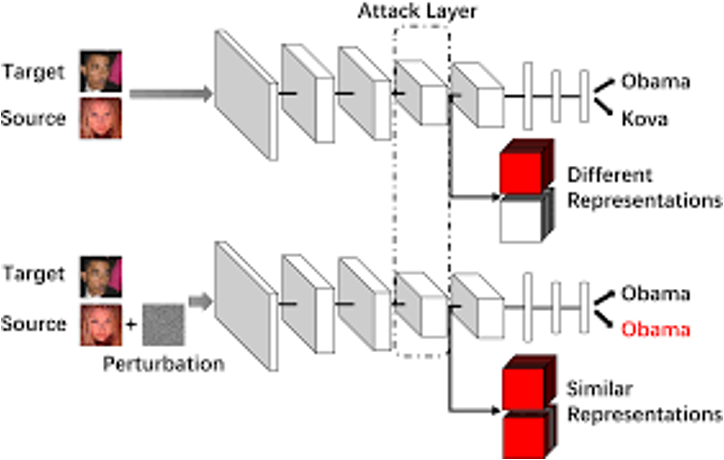
\includegraphics[width=\textwidth]{img/consequence.png} % Replace with actual image path
        \end{minipage}
        \begin{minipage}{0.35\textwidth} % Adjust width as needed
            \caption{Examples of the Consequences of Transfer Learning Attack.}
            \label{fig:transfer-attack}
        \end{minipage}%
    \end{figure}
\end{frame}

% %------------------------------------------------
\begin{frame}{How to Prevent Transfer Learning Attacks?}
    \begin{columns}
        \column{0.5\textwidth}
        \textbf{Key Preventative Measures:}
        \begin{itemize}
            \item Secure Training Data
            \item Model Isolation
            \item Knowledge Distillation
            \item Differential Privacy
            \item Adversarial Training
        \end{itemize}
    
        \column{0.5\textwidth}
        \textbf{Additional Techniques:}
        \begin{itemize}
            \item Data Augmentation
            \item Ensemble Methods
            \item Post-processing and anomaly detection
        \end{itemize}
    \end{columns}
    \begin{figure}[h]
        \centering
        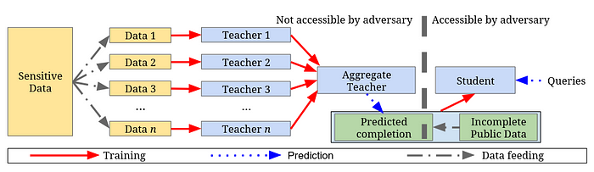
\includegraphics[width=0.53\textwidth]{img/how-to-prevent.png}
        \label{fig:how-to-prevent}
        \caption{Differential privacy as a protection to Transfer Learning attacks}
    \end{figure}
\end{frame}



% \begin{frame}
% 	\frametitle{Text paragraph}
%     Lorem ipsum dolor sit amet, consectetur adipiscing elit. Nullam ipsum velit, cursus quis ligula eu, malesuada aliquet massa. Quisque non convallis felis, a auctor eros. Etiam sit amet turpis a sapien pulvinar malesuada quis quis nisi. Quisque scelerisque volutpat ligula vel mollis. Nam sit amet tristique erat, sit amet cursus mi. 
% \end{frame}

% %------------------------------------------------

% \begin{frame}
% 	\frametitle{Text with enumerate }
%      Lorem ipsum dolor sit amet, consectetur adipiscing elit:
%     \begin{enumerate}
%         \item Lorem ipsum dolor sit amet.
%         \item Lorem ipsum dolor sit amet.
%     \end{enumerate}
	
% \end{frame}

% %------------------------------------------------

% \begin{frame}
% 	\frametitle{Text with itemize}
%      Lorem ipsum dolor sit amet, consectetur adipiscing elit:
%     \begin{itemize}
%         \item Lorem ipsum dolor sit amet.
%         \item Lorem ipsum dolor sit amet.
%     \end{itemize}
	
% \end{frame}

%------------------------------------------------

